\chapter{Fun with Data!}

\section{Quick Start}

Installing R or Python is not very complicated and both programs are completely free and open source and run on Windows, Mac, and Linux.
In fact, in the next chapter we will take you through the steps to install both programs.
However, to get started quickly and to make sure you are not slowed down by technical problems,
we will now use \emph{docker images} that you can easily run and that include all libraries that we use in the examples.

Throughout the book, you can choose to use either R or Python, or use both side-by-side.
Of course, if you already have your choice of R and/or Python installed on your computer, you can skip directly to \refsec{fun.simple}. 

\subsection{Installing the R docker}

\paragraph{Linux} To install and run the R docker on linux, open a terminal and give the following commands:
(please change the password to something a little bit more secret!)

\begin{terminal}
sudo apt install -y docker.io
sudo docker run --name rstudio -d -p 8787:8787 -e PASSWORD=password \
     rocker/tidyverse:3.6.1
\end{terminal}


\paragraph{Mac}

\paragraph{Windows} 

To check whether the installation worked, open a browser and go to \url{http://localhost:8787}.
You should see an RStudio Server login prompt like shown in \reffig{fun.rstudio.signin}:

\begin{figure}
\centering
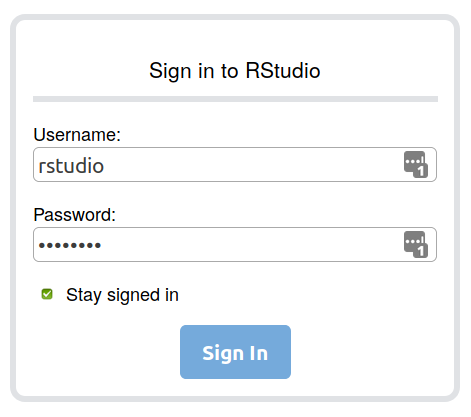
\includegraphics[width=0.4\linewidth]{figures/ch02_rstudio_signin.png}
\caption{RStudio Server Signin screen.}
\label{fig:fun.rstudio.signin}
\end{figure}

After entering the username \texttt{rstudio} and the password you used above (simply \texttt{password} if you copied the instructions without changing it),
you should see an RStudio Server screen such as displayed in \reffig{fun.rstudio}.
On the left hand side, you can see the console where you can directly give commands like the calculation for \texttt{1+1} I entered.
On the right hand side, you can see your environment which shows which data you have loaded (currently empty), and the list of files in the current folder
(currently mostly empty). 

\begin{figure}
\centering
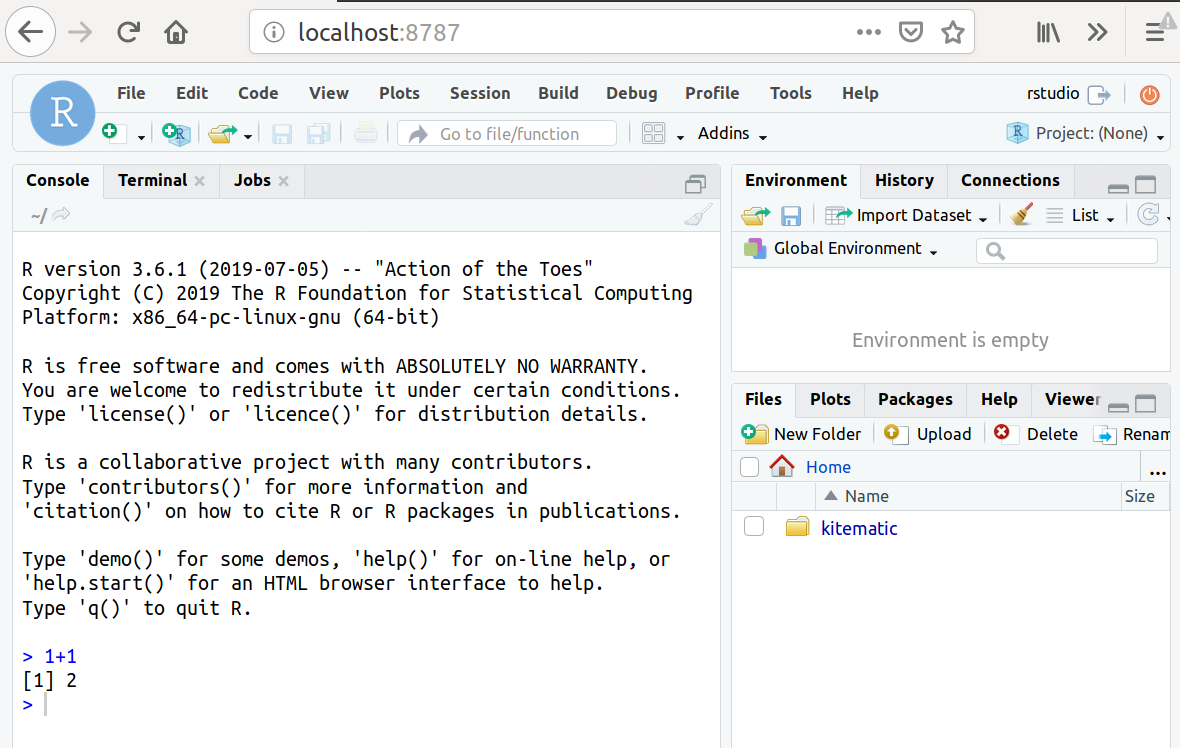
\includegraphics[width=0.7\linewidth]{figures/ch02_rstudio.png}
\caption{RStudio Server: Ready for Action}
\label{fig:fun.rstudio}
\end{figure}

\section{Simple Visualization} \label{sec:fun.simple}

\section{Exploring texts, networks, and maps}
